%==========================================================================================================================
% (c) Vojtěch Kulička, 2010
\linenumbers
\chapter{Introduction}
Human is a social creature and likes to chat, share feelings and ideas. At first we managed to do so by making simple sounds. Those sounds later on developed into words. Then much later the human race started to feel the need to record what we were thinking. We made up symbols and started to write. As the society grew and spread, we wanted to communicate with people from other tribes and villages. At first we would travel and use spoken words, but as the distances grew we figured we can have our thoughts delivered in writing. Mail was born. In 1844 telegraph was invented by Samuel Morse followed by telepthone in 1874 by Alexander Graham Bell. And finally in 1969 the Internet was created. All of these inventions aimed to provide means of communication to satisfy the needs of the evolving society.  

In the early days of the Internet email was the main means of communication. And just like regular mail people would have their electronic mailboxes to which the emails were delivered. Email was a huge step forward for it provided a way to almost instantly deliver text from one place to another regardless of the distance for free. The main disadvantage of email is that people had to check their mailboxes read new mail and then reply. It is just neither fast nor convenient enough for team cooperation when team members are far apart. For those and other purposes like chatting Instant Messenger programs were introduced.    

An IM program offers realtime communication between two people via text messages that are delivered from one user to another instantly. Instant messangers became very popular and started adding on features like multiuser chat, various games and most importantly VoIP(Voice over IP) support. VoIP capable IM like skype have become extremely popular at first for making it possible for people to call each other for free over the internet. Later video conferencing capability was added, so you could talk and see you colleague at the same time. One more thing comes in extremely handy when working in a team - a whiteboard.

At this time there is no usable IM providing VoIP and shared whiteboard for GNU/Linux. This thesis aims to add VoIP support to an existing XMPP client with shared board called Makneto. Makneto was created by Jaroslav Řezník as a master's thesis in 2008. At this point it is using iris library for XMPP communication. The shared board data is also transferred over XMPP. One of the goals of this thesis is to port Makneto to telepathy, which is now a very reliable and robust library for communication for numerous protocols.  

The following chapter~\ref{chapter:makneto} gives a detailed description of the current version of program Makneto. We will find out about it's architecture, strengths and weaknesses. 

Chapter~\ref{chapter:xmpp} focuses on XMPP/Jabber communication protocol. It talks about it's features and limitations. The chapter contains concrete examples that give the reader an idea of how it works and is it so popular.

Chapter~\ref{chapter:telepathy} is about Telepathy communication framework, how it works, what it consists of. There is also a description of a IM client application Empathy based on Telepathy. 

Current audio and video streaming protocols are listed and discussed in chapter~\ref{chapter:existing-solutions}. Based on this chapter a suitable protocol is chosen for the implementation. This chapter also talk about VoIP and what should the implemantator have in mind when writing a VoIP application.

The port to Telepathy and new Makneto's architecture are in chapter~\ref{chapter:port-to-telepathy}. It talks about design decisions and reasoning behind them. 

Chapter~\ref{chapter:voip-implementation} explains how was the VoIP implemented, what problems were encountered and what is the result.  

% =========================================================================================================================
% =========================================================================================================================

\chapter{Makneto}\label{chapter:makneto}
The collaborative application Makneto is the main topic of this chapter. First we take a look at the architecture and what it is based on. The following section explains why port Makneto to Telepathy and add VoIP. The main sources are \cite{makneto,qtBook,SVGtiny}. 
   
\section{Current architecture}
Makneto is an instant messenger with a shared board capability. It was written by Jaroslav Řezník as his master's thesis in 2008. Makneto is written in C++ using Qt version 4 and KDE 4 libraries. Qt is a application framework. It extends C++ and adds dynamic functionality like signals and slots mechanism or property system. Signals and slots are used instead of callback function, because they are as opposed to callback functions type-safe. The dynamic property system allows objects to have properties added at runtime without previous specification in their header file. In order to use the extended functionality the objects must directly or indirectly inherit QObject, which all Qt classes are derived from. These mechanisms also require to be compiled by the Meta Object Compiler before any standard C++ compiler.

Qt runs on all major computer platforms like GNU Linux, Microsoft Windows and Mac OS X. Moreso it is supported by mobile device platforms such as Symbian and Microsoft Windows Mobile. There is also a port to Google Android called Lighthouse. It was developed by company named Trolltech and was available under two licenses. First was a commercial license allowing companies to write proprietory applications for a fee. Second was GNU General Public License, which was of course free. Thanks to the commercial license the Qt documentation is one of the best among any software available under GNU GPL. In june 2008 Troltech was acquired by Nokia. Nokia decided to make the source code available so that anyone could contribute. In January 2009 with the release of Qt 4.5 another licensing option was added - Lesser General Public License \cite{qtBook,Qt}.

Besides Qt Makneto utilizes functionality provide by KDE 4 \cite{KDE} libraries, which makes Makneto unable to run on a different operating system than GNU Linux. KDE is a desktop environment created by Matthias Ettricht in 1996 for he felt the need for a good quality window manager for Linux. KDE is currently in version 4, which brought great features. There is a new desktop called Plasma, which allows users to display widgets called plasmoids directly on the desktop. That allows users to have a TODO list, calendar, translator, weather forecast, system monitor and much more right in front of them on their desktops without having launch any of those to get the information they need. It makes users' work eesier and more efficient. KDE and GNOME are the most common window manager in Linux. GNOME offers stable useful environment and is influenced mostly by large businesses using it. KDE is more flexible and works more with the look and feel.

Makneto communicates using XMPP/Jabber protocol implemented in Qt-based C++ library called Iris. All of the Iris is primarily used by Psi instant messenger. It's development is still quite active and it supports all of Jabber's key features. Iris' downside is very poor documentation. It's wiki is very brief and all to all gives one example. The only way to find out how it works is browsing through Psi code \cite{irisWiki}.

Makneto's shared whiteboard is based an official extension of XMPP SVGWB by Joonas Govenius \cite{SVGWB}. SVGWB is implemented in Psi and Makneto utilizes their code. SVGWB defines all the necessary actions like whiteboard session initianion including invitation and mainly how to send and receive information about the grahical objects using XMPP text messages. The actual graphical object representation is defined by SVG \cite{SVG}(Scalable Vector Graphics) by W3C. SVG describes graphics objects using vectors in XML format. Makneto uses just a subset of SVG called SVG Tiny \cite{SVGtiny} as it does not need all of the features of SVG. Tiny SVG describes two-dimensional vector graphics and raster graphics and multimedia. To sum up Makneto's whiteboard features, it allows you to draw lines, rectangles, elipses, circles, sketch using a paintbrush and input images in jpg and png formats. Graphical objects are resizeable, can be rotaded and copied.  

\begin{figure}[ht]
\begin{center}
	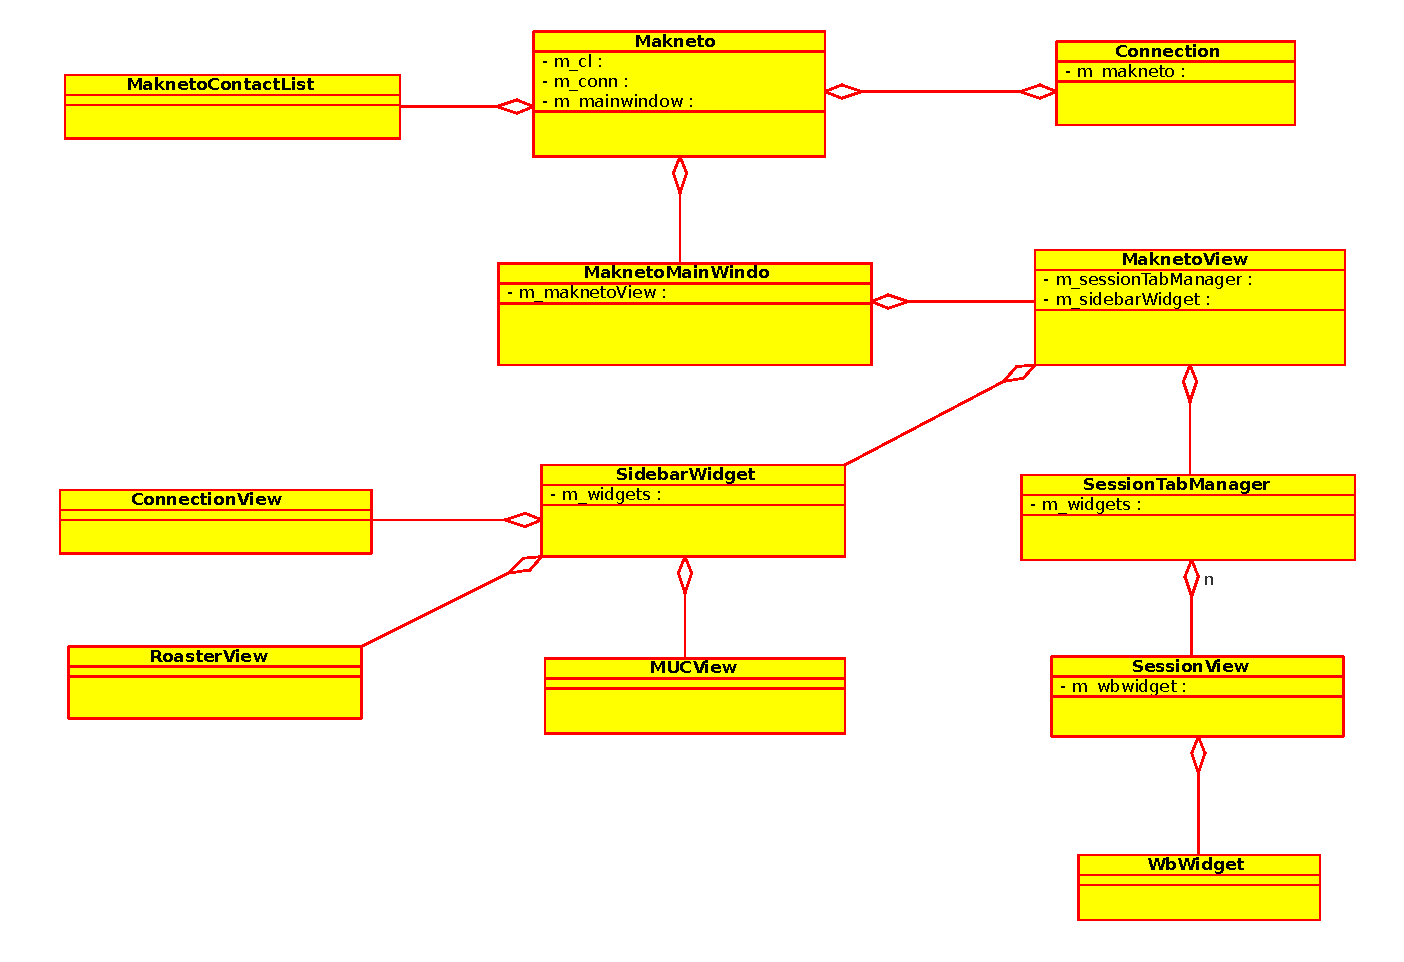
\includegraphics[width=15cm]{fig/makneto-orig-class-diagram.pdf}
	\caption{Makneto class diagram}
	\label{fig:makneto-original-class-diagram}
\end{center}
\end{figure}

Makneto runs in one window, which you can see in figure~\ref{fig:makneto-original} and is represented by class \verb|MaknetoMainWindow| as shown in the class diagram in figure~\ref{fig:makneto-original-class-diagram}. User's contact list is on a panel on the left hand side as a part of stacked widget along with MUC\footnote{Multi-User Chat} tab and tab for controlling presence. The whiteboard and chat session are initiated through the contact list. Makneto handles more session at once each in a separate tab. Each tab is represented by a \verb|SessionView| object and the whiteboard within it by WbWidget. The subject to change is class \verb|Connection| that is built on top of iris library. Using the application is very comfortable although it from dies time to time.


\begin{figure}[ht]
\begin{center}
	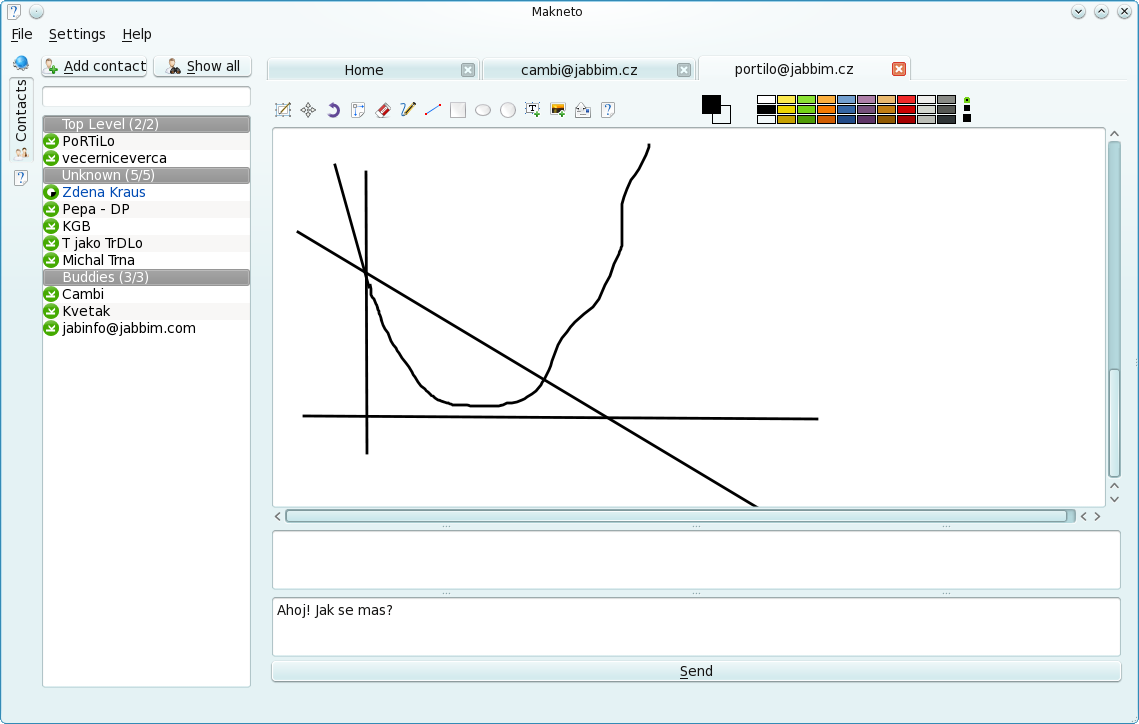
\includegraphics[width=15cm]{fig/makneto-original.png}
	\caption{Makneto before any work was done on it.}
	\label{fig:makneto-original}
\end{center}
\end{figure}


\section{Motivation for porting and adding VoIP support}
Makneto has a potential to become a great collaboration tool. The tasks of today are more and more dificult so the need to solve the task in teams is greater and greater. Especially in comupter science the teams are ofter from all over the world and it is important to discuss current issues. Meeting in person is not an option and that is where Makneto comes in. The shared whiteboard is very useful for sharing thinkmaps and visualising problems and solutions, but the days when people had the time and patience to write are gone. Everybody wants to talk these days.  

Makneto is at this point has couple design flaws. First it uses iris library for communication in XMPP network. Iris is very poorly documented and every change in the implementation would reflect in Makneto. Second Makneto depends on KDE libraries, which at this point is not necessary. Getting rid of this dependancy will help increase Makneto's portability. 

The current implemenation of Makneto is UI and backend in one large application. The goal is to separate the backend and UI. Backend will take care of communication. That means text messaging, shared whiteboard and after this thesis is finished also VoIP. Backend will use communications framework telepathy described in the following chapter. Telepathy supports various protocols as well as voice and video calls. Makneto will be able to use XMPP, ICQ, IRC, MSN etc. with one implementation of a client.

Frontend shall be a subject to change based on target device. Makneto for PC will have a Qt4 frontend and Makneto for smartphones and tablets will use the Qt Quick UI. With rapidly increasing number tablets and smartphones made and sold it would be shame not to plan to support them.  



% =========================================================================================================================
% =========================================================================================================================

\chapter{XMPP}\label{chapter:xmpp}
This chapter talks about Extensible Messaging and Presence Protocol \cite{xmpp}, it's history, key features and usage. The information is mailny acquired from \cite{xmppBook,xmppCoreRFC,xmppIMRFC}.

In 1999 Jerremie Miller created protocol called Jabber. Jabber was an open protocol based on XML as opposed to existing protocols like ICQ \cite{ICQ} or AIM \cite{AIM}, which were proprietory and owned and controlled by private companies. The first attemp to make Jabber a standard failed. The second attempt did not use the name Jabber, but eXtensible Messaging and Presence Protocol instead. IETF\footnote{Internet Engineering Task Force} approved and XMPP was standardized in 2004 in RFC 3920 and RFC 3921 called XMPP Core and XMPP IM respectively. Development of XMPP is still active as it is based on XML it is possible to add functionality without jeopardising the compatibility of existing implemenstations.      

XMPP is a robust, scalable, secure, open and extensible protocol that has been well tested over the years passing all of the test without any sign of trouble. It has been very well though out and altogether it is a great protocol. The description given bellow is in some of the parts simplified. Full description is out of the scope of this thesis.   

\section{XMPP protocol}
XMPP is defined in \cite{xmppCoreRFC} and \cite{xmppIMRFC}, which describe all the key features of the protocol. Authors of XMPP aim for a scalable, extensible and in every way powerful protocol. Years later with XMPP still around and more and more popular we can safely say they succeeded. The key features of XMPP include:

\begin{itemize}
	\item \textbf{Decentralized architecture} - XMPP network does not rely on one server. The network consists of servers and clients. Every client may run his or her own server. XMPP server registers clients and communicates with other servers much like with email(see figure \ref{fig:xmpp-decentralized-architecture}). A client often wants to communicate with another client on a different server. In such case other client's server is looked up and the message forwarded. If a client is not satisfied with the server he or she registered with he or she may simply register with a different server or run his or her own. There is also no way to take the whole network out with DoS\footnote{Denial of Service} or DDoS\footnote{Distributed Denial of Service} attack. There simply is not a small number of target to attack.    
	\item  \textbf{Open nature} - XMPP is an open standard that can be used by anyone without having to pay, sign any agreement or behave by any restrictive policies. Also it's fate is not in hands of one company but rather in the hands of everyone. Anyone who wishes to contribute can do so by cooperating with XMPP Standards Foundation. 
	\item \textbf{Extensibility} - thanks to XML based nature of XMPP it is very simple to add new features without discontinuing support of the old ones. This feature makes XMPP very flexible for it can easily add new functionality and it has been already done couple times.  
	\item \textbf{Security} - with built-in support for TLS and SSL there is no need to worry that the messages might be read by a third person using man in the middle attack. Companies using XMPP for communication inside their network might run their server localy with no access to the outside world.  
\end{itemize}

\begin{figure}[ht]
\begin{center}
	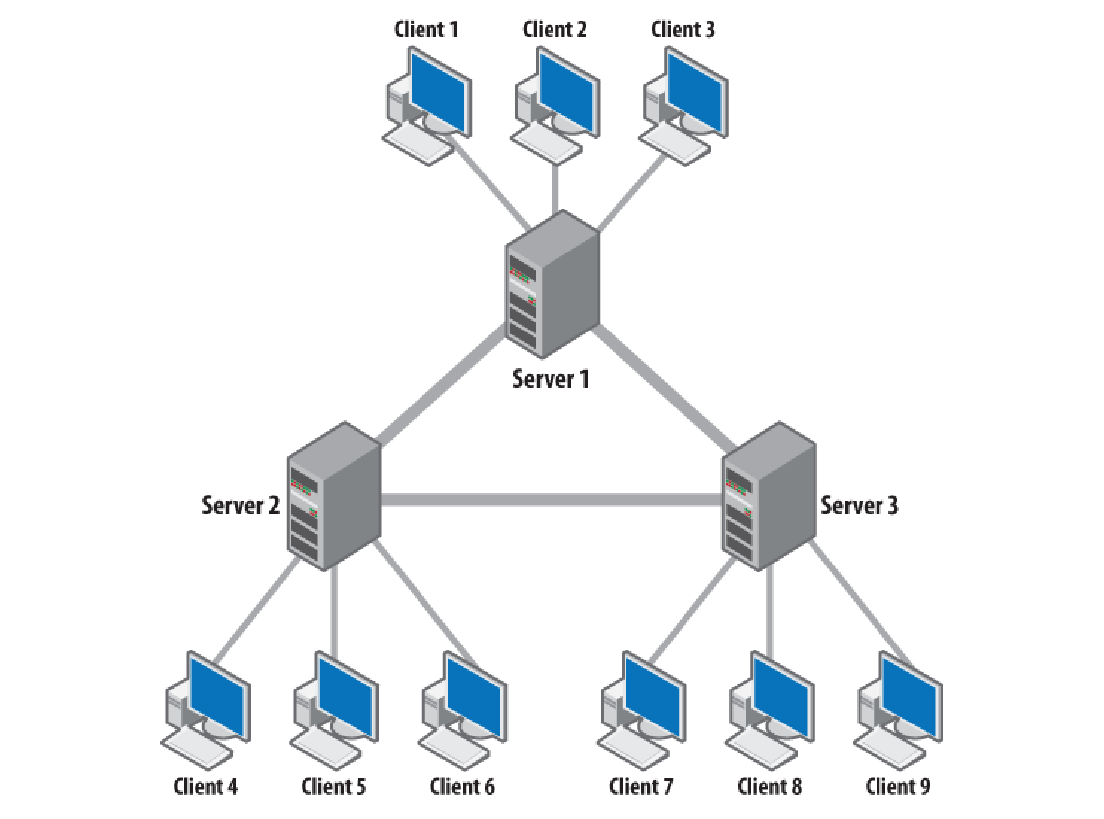
\includegraphics[width=10cm]{fig/XMPP-decentralized-architecture.png}
	\caption{XMPP decentralized architecture \cite{xmppBook}}
	\label{fig:xmpp-decentralized-architecture}
\end{center}
\end{figure}

Now let's look at the protocol and how to use it. 

\subsection*{Client-server communication}
XMPP is basicaly streaming XML documents. The stream is an unbounded XML document which contains another XML documents from both client and server. The XML documents enclosed in the stream tags with a depth of 1 are called stanzas. Stanza is a basic unit of communication like a packet. The following stanzas are defined:

\begin{itemize}
	\item \textbf{message} - used for getting information from one place to another in a push manner. The message stanza is not acknowleged and no answer is expected. It is used for instant messages, alerts, notifications, groupchat etc. The nature of the message is specified by \verb|type|.  
	\item \textbf{presence} - stanza for acquiring another user's presence. XMPP honors usess' privacy and to get someone's presence status he or she need to authorize it first by adding the querier to his or her contact list. There are several types of presence just like in any other IM protocol.     
	\item	\textbf{IQ} - is an abbreviation for Info/Query. This stanza is used for everything else. IQ works on question-answer basis. It is used for example for getting remote client's capabilities. IQ stanza must always receive a reply. 
\end{itemize}

First a TCP connection is established between client and server. Once established a stream is opened by client by sending the server \verb|<stream>| tag. There is an example of opening a stream below: 

\begin{figure}[h]
\lstset{language=XML,caption={Opening communication with server}, label=lstXmppBeginCommunication}
\begin{lstlisting}
<?xml version='1.0' encoding='UTF-8'?>
<stream:stream 
	xmlns='jabber:client' 
	xmlns:stream='http://etherx.jabber.org/streams' 
	to=\"jabbim.cz\" 
	version=\"1.0\">
\end{lstlisting}
\end{figure}

Server answers with a second stream back to the client, which is shown in the piece of XML code that follows. 

\begin{figure}[h]
\lstset{language=XML,caption={Server's reply to client's opening stream}, label=lstXmppBeginCommunicationServersAnswer}
\begin{lstlisting}
<?xml version='1.0'?>
<stream:stream 
	xmlns='jabber:client' 
	xmlns:stream='http://etherx.jabber.org/streams' 
	id='856661962' 
	from='jabbim.cz' 
	version='1.0' 
	xml:lang='en'>
\end{lstlisting}
\end{figure}

The next step is to negotiate properties of the stream. The server sends an XML enclosed in \verb|stream:feature| tags, informing the client about features it supports. The most important property is by far encryption and authentication. Preferred encryption method is TLS, but SSL is also an option. However some servers may require usage of TLS. TLS is recommended for both client-server and server-server communication. Authentication is a key responsibility of the server. The server must ensures that users attempting to connect to it are who they say they are. The server acts as a gateway to the entire network and must not allow identity spoofing. Authentication is done via SASL\footnote{Simple Authentication and Security Layer} and options supported by the server are enclosed in \verb|mechanism| tags. The example, where server supports TLS and SASL using PLAIN text or MD5 is shown below:   

\begin{figure}[h]
\lstset{language=XML,caption={Server sends supported encryption options}, label=lstXmppServersEncryptionOpts}
\begin{lstlisting}
<stream:features>
	<starttls 
		xmlns='urn:ietf:params:xml:ns:xmpp-tls'/>
	<mechanisms xmlns='urn:ietf:params:xml:ns:xmpp-sasl'>
		<mechanism>
			PLAIN
		</mechanism>
		<mechanism>
			DIGEST-MD5
		</mechanism>
	</mechanism>
	...
</stream:features>
\end{lstlisting}
\end{figure}

Once stream parameters are set, client can request presence, set his or her own presence and communicate with other clients. Sending a message to a fellow user is accomplished via \verb|message| stanza and may look like this:

\begin{figure}[h]
\lstset{language=XML,caption={Chat message}, label=lstXmppChatMessage}
\begin{lstlisting}
<message 
	from='vtheman@jabbim.cz'
   to='kuba86@jabber.cz'
	xml:lang='en'>
	<body>Hey, how are you?</body>
</message>
\end{lstlisting}
\end{figure}

It must include \verb|to|, \verb|from| attributes and \verb|body| opening and closing tags. The first specifis who the message is addressed to using a Jabber ID. Jabber ID consists of \newline\verb|user name @ domain name [/ resource]| and many people mistake for email address because the resource is optional. Resource was added to JID to allow user to connect from different device/locations without having to log out. An example of resource is \verb|home| or \verb|work|. A simple Jabber ID is \verb|vtheman@jabbim.cz|. Attribute from naturaly contains a jabber ID as well, but this time an ID of the sender. The \verb|body| element contains the actual message. 

Next stanza is presence and it is needed for following presence of the contacts in the users' roster. To get presence of a user he or she must approve of it. Once user has been authorized to get another users presence they have both subscribed to get each other's presence. After connecting to the server a user sends initial presence stanza: \verb|<presence/>|. From that moment on the server takes care of the presence. Whenever the user's presence changes, it sends notification to all subscribers in the user's roster. Similarly if someone else's presence changes the user gets notified by his or her server. 

\begin{figure}[h]
\lstset{language=XML,caption={Presence publication}, label=lstXmppPresence}
\begin{lstlisting}
<presence from="vtheman@jabbim.cz" to="kuba86@jabber.cz">
	<show>dnd</show>
	<status>Working on my thesis!</status>
</presence>
\end{lstlisting}
\end{figure}

Presence stanza contains elements \verb|show| and \verb|status|. \verb|show| can be either \verb|chat| meaning available and ready for chat, \verb|away| meaning the user is not at the PC at the moment, \verb|xa| indicates the user will be gone for a longer period of time and finaly \verb|dnd|, which stands for do not disturb.  

The last of stanzas is Info/Query shortly IQ. IQ is very similar to HTTP in methods and in the query-answer nature. IQ queries use method \verb|get| for requesting information and method \verb|set| for making requests based on provided information. Answer to a query is IQ stanza of type \verb|result| and contains information requested by \verb|get| method or acknowledge in case of \verb|set| method. The last type of IQ is \verb|error| and is used to indicate that something went wrong. A good example of an IQ stanza is acquiring a roster: 

\begin{figure}[h]
\lstset{language=XML,caption={Requesting roster from server}, label=lstXmppRoster}
\begin{lstlisting}
<iq type="get">
	<query xmlns="jabber:iq:roster"/>
</iq>
\end{lstlisting}
\end{figure}

And the server replies with:

\begin{figure}[h]
\lstset{language=XML,caption={Roster sent by the server}, label=lstXmppRosterAnswer}
\begin{lstlisting}
<iq type="result">
	<query xmlns="jabber:iq:roster">
		<item jid="kuba86@jabber.cz"/>
		<item jid="rezza@jabber.cz"/>
		<item jid="imlich@jabber.fit.vutbr.cz"/>
	</query>
</iq>
\end{lstlisting}
\end{figure}

The stream ends with \verb|</stream>| tag and that means end for the communication. 

\subsection*{XMPP Extensions}
As mentioned earlier XMPP is easily extensible due to it's XML based architecture. XMPP extensions are published by XSF\footnote{XMPP Standards Foundation} as XEP\footnote{XMPP Extension Protocol}. Basic XMPP functionality is defined in the RFC 3920 and RFC 3921 and every XMPP server and client ought to implement it. Functionality described in XEP however is optional. These are the most popular extensions:
\begin{itemize}
	\item{\bf Multi-User Chat} defined in XEP-0045 \cite{xepMUC} allows users to create virtual rooms just like in IRC, invite their contacts to join the room and thus communicate with multiple people.
	\item{\bf Service Discovery} registered as XEP-0030 \cite{xepServiceDiscovery} defines a way of findit out what capabilities have one's contacts.
	\item{\bf Entity Capabilities} defined in XEP-0115 \cite{xepCapabilitiesAdvertisement} adds client's capabilities to presence information, so that if a XEP-0115 capable client requests presence it receives a list of supported features as well.
\end{itemize}

There are tens of extensions either standardized of waiting for becoming a standard defining various handy features.

\section{Jingle}
XMPP Extension defined in XEP-0166 \cite{xepJignle} known as Jingle is a signaling protocol that initiates, manages and terminates media sessions via XMPP. Jingle was first used in Google Talk \cite{googleTalk} for Voice call signaling in 2005. The idea was to use an existing XMPP comunication channel to setup a peer-to-peer media session that uses a diferrent means of transporting data, e.g RTP\footnote{Real-time Transport Protocol} for voice or video and TCP for file transfer. 

Figure \ref{fig:xmppJingleDataFlow} shows how the protocol works. Session initiation starts when the initiator sends \verb|session-initiate| with Application type, e.g voice call, and Transport method, e.g UDP are described. As you can see in the figure Jingle uses an IQ stanza so the initiator immediately receives a IQ result acknowledging the invitation reception from the responder. Next all the necessary application type and transport type parameters of the session are negotiated. In case of voice call the application type paraneters might be audio codec and sampling frequency. Transport type parameters include the peers' IP addresses and ports and transport method. When all the parameters have been setup the responder either accepts or declines the invitation. If accepted the data start flowing between the two peers just as it was agreed during the initiation phase. Jingle can also be used to adjust parameters of an existing session if necessary. And finaly one of the peers sends the other \verb|session-terminate| to end the session. 

\begin{figure}[ht]
\begin{center}
	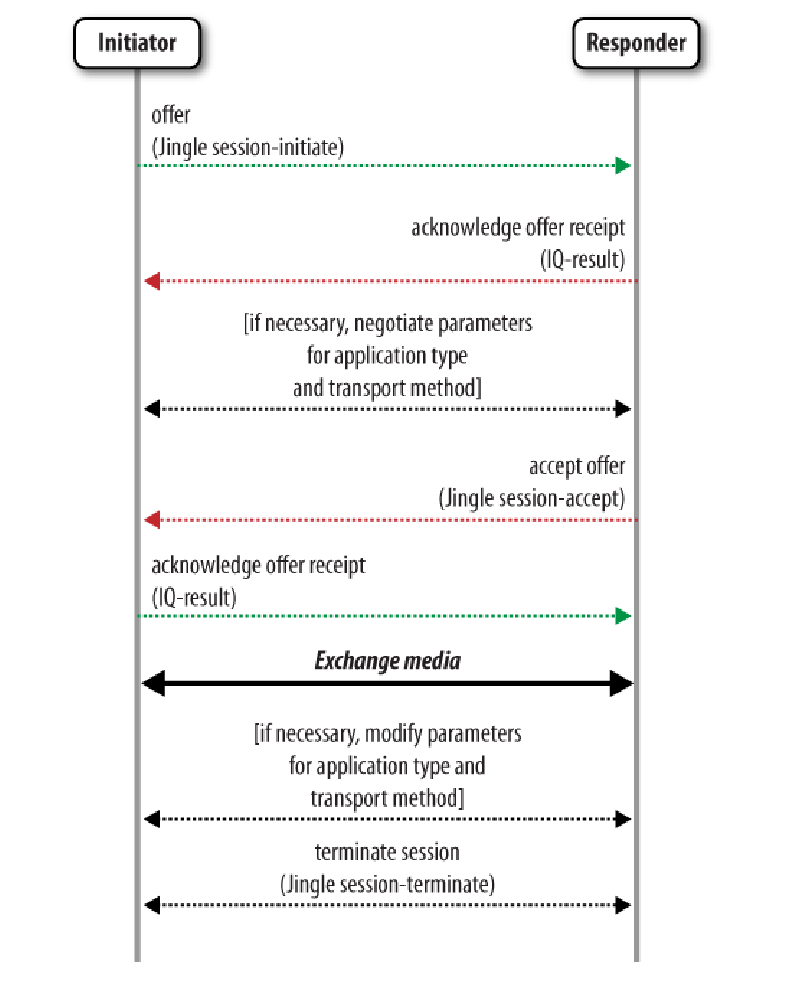
\includegraphics[width=10cm]{fig/xmpp-jingle-flow.png}
	\caption{Data flow in media session initiation, management and termination using XMPP Jingle \cite{xmppBook}}
	\label{fig:xmppJingleDataFlow}
\end{center}
\end{figure}


% =========================================================================================================================
% =========================================================================================================================

\chapter{Telepathy}\label{chapter:telepathy}
In this chapter the framework to which Makneto shall be ported is looked at. First basic terms and basic idea of how is the framework designed what can it do. Then we describe D-Bus and the relationship with Telepathy and have a detailed look at components of Telepathy. Finally we talk about an existing client built on Telepathy. The chapter takes information mainly from \cite{TPWiki, dbus}. 

Telepathy \cite{telepathy} is a modular communications framework for building real-time communication applications. It supports numerous communication protocols as plugable backends e.g XMPP/Jabber(telepathy-gabble), SIP(telepathy-sofiasip), MSN(telepathy-butterfly), etc. Each of telepathy's components runs in a separate process as desktop service and communicates via D-Bus. The components are shared by telepathy clients. For example if there are two clients using XMPP they both use the same instance of telepathy-gabble. To get a better idea of how this concept works take a look at figure ~\ref{fig:telepathyArchitecture} \cite{TPWiki}.

\begin{figure}[ht]
\begin{center}
	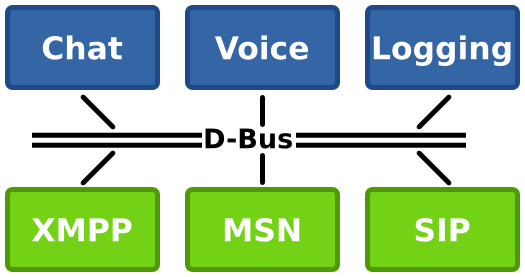
\includegraphics[width=7cm]{fig/telepathy-architecture-overview.png}
	\caption{Telepathy architecture \cite{TPWiki}}
	\label{fig:telepathyArchitecture}
\end{center}
\end{figure}


There are several features making telepathy very useful as a communications framework.

\begin{itemize}

	\item {\bf Robustness} - all the components are independent. If one crashes, others will not be affected

	\item {\bf Ease of development} - the components can be replaced without having to stop the service 

	\item {\bf Language independence} - since telepathy components use D-Bus for communication among themselves, any language that has D-Bus binding might be used to write them

	\item {\bf Desktop independence} - D-Bus is present in both main Linux window managers GNOME and KDE, so the same telepathy components could be backend for appropriate frontends.

	\item {\bf Code reuse} - the client applications do not have to worry about protocol specifics, which are handled by Telepathy. The client can use more protocols by making no or small alterations to the code.

	\item {\bf Connection reuse} - more than one Telepathy client can use the same connection simultaneously:
\end{itemize}

\section{Telepathy architecture}
Telepathy is a very powerful framework and as such it is also complicated. To successfuly write programs using Telepathy we need to know what telepathy consists of and what it is based on. This section tries to put all the terms into context of this thesis.  

\subsection*{D-Bus}
D-Bus is a kind of inter-process communication. It allows two applications running in different processes, written in different programming language communicate. More so these applications may communicate directly, without having to go through message bus daemon. There two types of D-Bus. First is a system bus used for events such as ``USB device disconnected'' or ``printer out of paper.'' Second type is per-user-login-session bus, which is used by user applications. D-Bus low level API is represented by libdbus and it requires XML parser(libxml or expat) to work. Higher level language bindings such as Qt, GLib, Java etc. are built on top of libdbus and offer more convenient way of using D-Bus, although they add more dependencies \cite{dbus,TPWiki}.

Each process that wants to communicate over D-Bus will need to use most the following depending on it's nature: 
\begin{itemize}
	\item {\bf Unique name} - is an unique id (e.g. 2.1) assigned by D-Bus daemon to the client application. Unique name is similar to a public IP address.
	\item {\bf Wellknown name} - is similar to a DNS name. If a process wants to make a service available to other processes it requsets a wellknown name. If another process wants to access the service it uses the wellknown name to do so. Wellknown name might look like this: org.freedesktop.Telepathy.ChannelDispatcher.    
	\item {\bf Object path} - is a path to an object that is exported by process running a service.
	\item {\bf Interface} - is a way of requesting a service using signals or methods. Each D-Bus client must register at least one interface and each interface provides at least one method or signal. Every interface needs to have to name like a wellknown name.  
	\item {\bf Method} - is impleneted in the object specified by object path and exposed in the interface for that object for other processes to use. 
	\item {\bf Signal} - is a D-Bus signal client process can connect to it's callback function. If a signal is invoked the callbacked function is called.
	\item {\bf Property} - is used for exposing D-Bus object's properties. To do so the objet must implement org.freedesktop.DBus.Properties interface.
\end{itemize}

The following figure \ref{fig:dbusArchitectureNames} shows an example of two programs connected to D-Bus to be able to communicate with each other. Program B provides a service called well-known name (\verb|org.freedesktop.foo.Bar|) and it's id is 1.3. Program A does not provide any service and thus does not need any well-known name. It just needs an id 1.2 to use other programs' services \cite{TPWiki}.

\begin{figure}[ht]
\begin{center}
	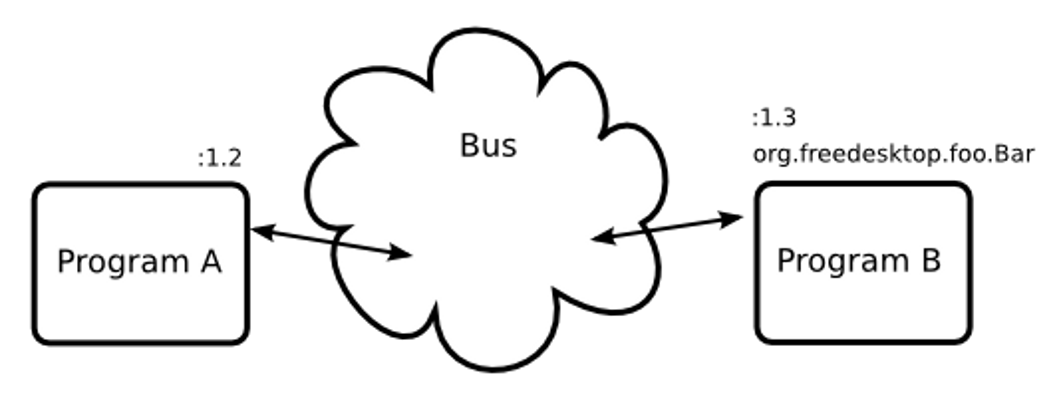
\includegraphics[width=11cm]{fig/dbus-architecture-names.png}
	\caption{D-Bus id and wellknown name example \cite{TPWiki}}
	\label{fig:dbusArchitectureNames}
\end{center}
\end{figure}


The figure \ref{fig:dbusArchitecture} shows an overview of all of the terms described above in a simple diagram.

\begin{figure}[ht]
\begin{center}
	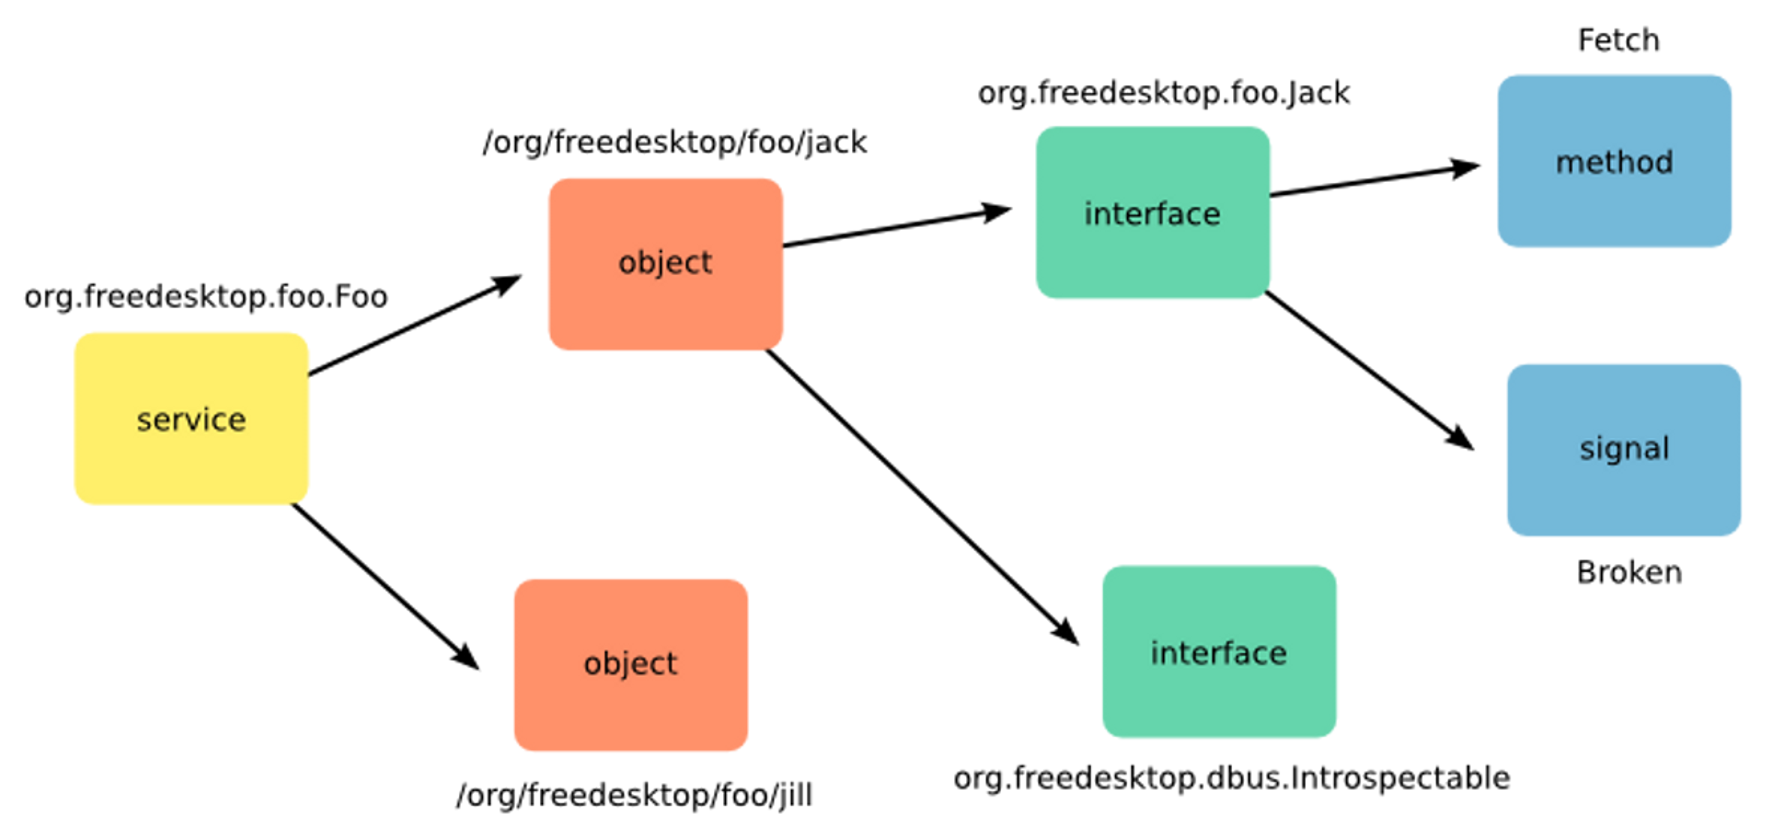
\includegraphics[width=15cm]{fig/dbus-architecture-overview.png}
	\caption{D-Bus architecture \cite{TPWiki}}
	\label{fig:dbusArchitecture}
\end{center}
\end{figure}

D-Bus is a key component of Telepathy framework. Telepathy supports many protocols all of which might provide different capabilites. For example IRC does not support avatars while XMPP does. Eventhough avatar feature is supported by XMPP protocol it might not be supported by the server we are connected to or by the opposite client in case of peer-to-peer connection. The available features are exposed by D-Bus Properties Interface. That is an easy way of determining the protocol, server or client capabilities \cite{dbus}.

\subsection*{Mission Control}
Mission Control is a Telepathy component that implements Account Manager and Channel Dispather and it's primary purpose is to encapsulate those two. There always only one running on the system. It is very important to check version running for they are backwards incompatible \cite{TPWiki}. For better understanding of the role of this and the following components have a look at figure~\ref{fig:telepathy-architecture}. It illustrates the relatioship among the the key components.

\subsection*{Account Manager}
Account Manager is responsible for handling accounts(e.g. XMPP, ICQ, MSN etc.). It is accessible by well-known name on D-Bus - \verb|org.freedesktop.Telepathy.AccountManager|. A client application first creates an account using the provided methods, supplying it with Connection Manager, protocol and display name. Account Manager creates and then as long as the Account is active maintains Connection to that Account. The Accounts are persistent and the next time the application runs it does not need to create them again. 

To create a Connection a Connection Manager is called by Telepathy. An Account may be valid or invalid and also enabled or disabled. Valid ones may establish a Connection, whereas invalid can't. Enabled and disabled property are user's way of telling the application which one should be ignored and which not. The lists of valid and invalid accounts is accessible via appropriately named methods as are the enabled and disabled.  \cite{TPWiki}.

\subsection*{Account}
Accounts are created via Account Manager. They are only created once and then stay on the system and can be accessed by any Telepathy clients. An active Account object registers with D-Bus and has an object path \verb|/org/freedesktop/Telepathy/Account/CM/PROTOCOL/ACCDN|. \verb|CM| stands for Connection Manager(e.g. gabble, salut, butterly, etc.), \verb|PROTOCOL| is substitution for a protocol name and \verb|ACCDN| is Account's Display Name. The Account object implements \verb|org.freedesktop.Telepathy.Account interface|. Features supported by this interface depend on the protocol used and the server-side software. 

The Account settings are done via i\verb|org.freedesktop.Telepathy.Properties| interface. All available attributes can be obtained by calling a single method provided by the properties Interface. The method is very convenient for it returns all the propeties at once in signle D-Bus call. Setting all properties at once works exactly the same. Some features are available via specified interface, e.g. avatar. Avatar used to be a property, but now it has it's own interface. The Interfaces property of the account lists all interfaces of additional features \cite{TPWiki}.

\subsection*{Connection Manager}
Connection Manager supplies Account Manager with Connections. It is not directly used by the client program. Account Manager requests connection for active accounts. There is always only one Connection Manager for each protocol running at any time.

Connection Manager is a protocol-dependent Telepathy component. Different protocols need different Connection Managers. For example if the client application wants to communicate using XMPP/Jabber it has to use Telepathy-gabble and for MSN Telepathy-butterfly is required. Some Connection Managers can communicate via more than one protocol, for example Telepathy-haze. To see what protocols are supported there is an appropriate method implemented by the Connection Manager \cite{TPWiki}.

\subsection*{Connection}
Connection represents an active protocol session. It is associated with an Account and is created by Connection Manager based on a request of the Account Manager. Connection implements org.freedesktop.Telepathy.Connection interface and additional interfaces depending on the protocol. List additional interfaces available can be retrieved by checking the Interfaces property. The most common interfaces are listed below\cite{TPWiki}:

\begin{itemize}

	\item {\bf Contacts} - used to get as much information about a contact as asked in one D-Bus call.

	\item {\bf Aliasing} - serves for setting aliases for contacts and checking if the contacts have changed their alias themselves. 

	\item {\bf Avatars} - interface to one of the most popular protocol features. Allows users to set their avatars and retrieve other users' avatars.

	\item {\bf ContactCapabilities} - retrieves capabilities of contacts' Clients to see what features they support. Checks for example for VoIP or file transfer support.

	\item {\bf Location} - lets user publish his or her current location as well as find out his or her contacts' whereabouts. 

\end{itemize}


\subsection*{Channel Dispatcher}
This component handles Channels incoming from active Connections of valid Accounts. Channel Dispatcher monitors available or activatable Telepathy Clients through D-Bus. Clients register with user's session D-Bus and provide a \verb|CLIENT\_NAME.client| file. Both of those serve as a way to publish Client's properties including a channel filter. The Channel Dispatcher based on these properties knows what kind of a client it is and what type of channels it is interested in (channel filter). If the Client is running then the properties are acquired via the Client interface. If the client is not running and is activatable then the .client file is used by Channel Dispatcher to pre-look up the properties and if they match the incoming Channel, the Client is activated. So providing the .client file only makes sense for activatable Clients.  

When a Channel comes in from one of the Connections Channel Dispatcher notifies appropriate Clients. There are three kinds of clients - Observer, Approver and Handler(see section~\ref{subsect:tpClient}). The Channel is dispatched to all Observers and all Approvers with a matching channel filter. The Approvers choose Handler to handle the Channel. Should the Client fail, Channel Dispatcher may recover from such error and look for another Handler \cite{TPWiki}.


\subsection*{Channel}
Channel allows the local client to exchange various kind of data with a remote server. It is associated with a Connection and always implements at least two interfaces. The first is \verb|org.freedesktop.Telepathy.Channel| and the second depends on the Channel type. Channels for text messaging will be of type Text and will implement \newline \verb|org.freedesktop.Telepathy.ChannelType.Text| interface. The following list shows most common types of Channels \cite{TPWiki}:

\begin{itemize}

	\item {\bf ContactList} - used to get information of contacts in user's contact list.

	\item {\bf Text} - designed for exhanging text messages. 

	\item {\bf Call} - used for VoIP and video calls. 

	\item {\bf FileTransfer} - Channel for sending and receiving files.

	\item {\bf ContactSearch} - is used when a user wants to find a contact on a server.

\end{itemize}

Channels are created using two methods - \verb|CreateChannel()| and \verb|EnsureChannel()|. These methods are implemented by both Channel Dispatcher and Connection. When calling either of those methods on Channel Dispatcher the resulting Channel will go through the procedure of looking for handler as described above. When using directly the connection the calling application must handle the Channel itself as the Channel Dispatcher will not interfere. It is also possible to supply the Channel Dispatcher with a preferred handler and thus achieve the same effect. It is better to use the Channel Dispatcher for if the client should fail it may dispatch the Channel to another handler \cite{TPWiki}.

Both of the methods provide a Channel. The difference between the two is that \verb|CreateChannel()| creates actual new Channel whereas \verb|EnsureChannel()| will attemp to reuse an existing Channel with the same properties. The first is typicaly used for file transfer and contact search and the latter for text, streamed media and contact list Channels \cite{TPWiki}.

\subsection*{Client}\label{subsect:tpClient}
Client is an application that wants to use Telepathy. It needs to register a well-known name in org.freedesktop.Telepathy.Client namespace, e.g. Empathy registers \newline org.freedesktop.Telepathy.Client.Empathy. Then it provides a .client file where purpose of which is described above. Telepathy defines three types of clients - Observer, Approver and Handler. All of these need to provide appropriate channel filter, e.g. Oberver provides ObserverChannelFilter. Based on the published filter the Channel Dispatcher dispatches an incoming Channel to the Client or not.\cite{TPWiki}  

Observers are called upon a creation of a new Channel. They monitor Channels and provide the acquired information to user. The observers have different functions based on the type of observed Channel, e.g. Text Channel observer might serve as a logger and FileTransfer observer as a file transfer progress monitor. Observer is must not interfere except for when the user interaction like hitting the cancel button in a file transfer progress window.\cite{TPWiki}     

Approver is a Telepathy Client that is supposed to accept the incoming Channel and decide, which Handler it is dispatched to. The Channel Dispatcher provides Approvers with a list of possible Handlers. Approver notifies the user of a new Channel and lets him or her decide whether to accept or reject it. Similarly the user is allowed to choose which Handler will handle the Channel. Handler might also be chosen by the Approver itself. Approver does not call methods just like the Observer. Calling methods is up to the Handlers. For example if there is an incoming file transfer the Approves lets user decide whether to accept it or not, but the AcceptFile method will be called by the chosen Handler \cite{TPWiki}.  

The last client is Handler. Handler does all the interaction with the Channel. A typical example of a Handler is chat-window. It displays messages and allows the user to send text messages back \cite{TPWiki}.  

\begin{figure}[ht]
	\begin{center}
	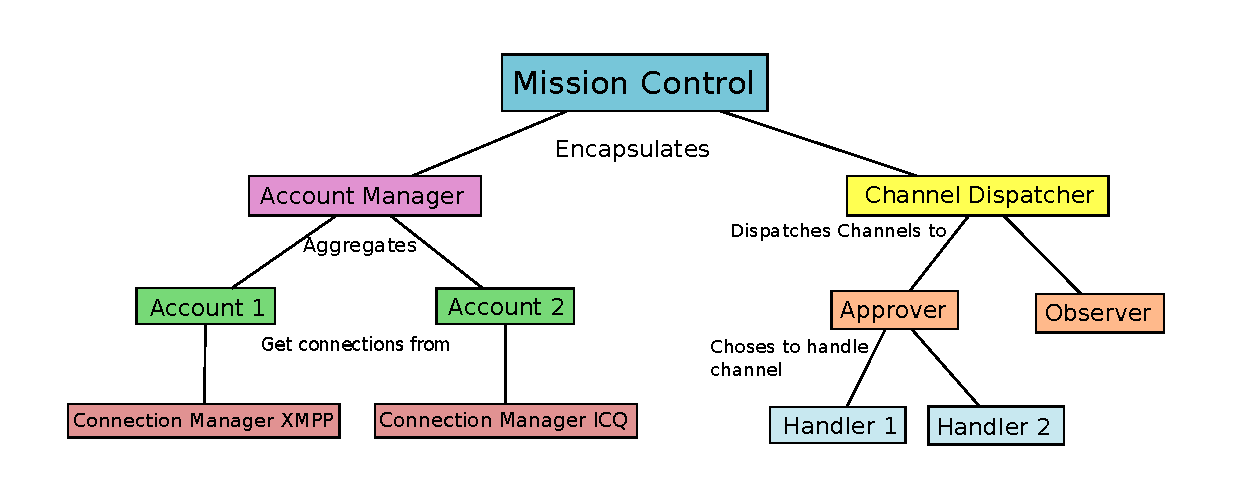
\includegraphics[width=15cm]{fig/telepathy-architecture.pdf}
	\caption{Simplified Telepathy architecture}.
	\label{fig:telelepathy-architecture}
\end{center}
\end{figure}

The figure \ref{fig:telepathyComponentsDbus} represents typical setting using Telepathy. There is one Accoun Manager and one Channel Dispatcher for those are unique in the system. Next we can see Connection Managers, which allow the clients use numerous protocols. In general the number of supported protocls equals the number of present ConnectionManagers. Finally there are clients, which may an Observer for logging, Approver and a Handler. But it as well may be three handlers. Also one client may represent Handler, Approver and Observer at the same time. All of these entities communicate va D-Bus.  

\begin{figure}[ht]
	\begin{center}
	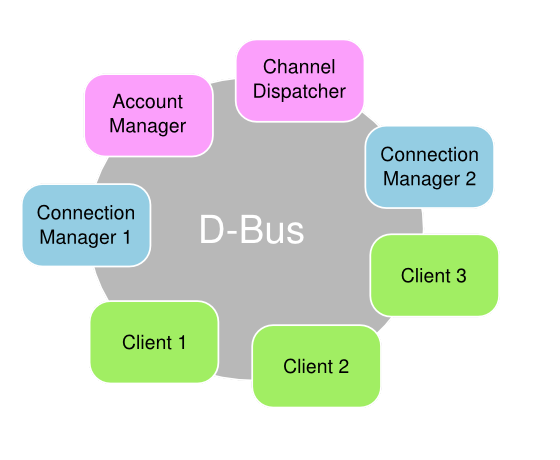
\includegraphics[width=9cm]{fig/telepathy-components-dbus.png}
	\caption{Telepathy components registered with user session D-Bus \cite{TPWiki}}.
	\label{fig:telepathyComponentsDbus}
\end{center}
\end{figure}


%\section{Telepathy language bindings}
%Telepathy clients may be written using language bindings. These bindings must provide D-Bus API. 
%Telepathy-glib, Telepathy-python
%Telepathy-qt4

\section{Empathy}
Empathy is a multiprotocol instant messaging application based on Telepathy. In the terms described above Empathy is a Telepathy client. It is written in python using Telepathy-python bindings. Empathy registers a well-known name with D-Bus and communicates with Telepathy components to provide the communication services. Empathy supports text messaging, file transfer, voice and video calls over various protocols. Supported protocol include Google Talk, XMPP/Jabber, MSN, IRC, AIM Facebook, Yahoo!, Gadu Gadu, and ICQ. For some of those protocols like Google Talk and XMPP voice and video calls implemented. The suppport of the protocols depend on Telepathy Connection managers installed. Additional functionality includes sharing users' whereabouts among themselves, automatic reconnection when internet connection is reestablished and automatic changes of presence to away and extended away.\cite{empathyGnome}

The current stable version of Empathy is 2.32.2 and it is a default communication application in GNOME releases since version 2.24 instead of Pidgin. Empathy also replaced Ekiga - program for voice calls and video-call. It became an ultimate free communication tool. Empathy's GUI is takes after Gossip, which is an older IM application for GNOME. 

% =========================================================================================================================
% =========================================================================================================================

\chapter{Existing solutions}\label{chapter:existing-solutions}
The first section of this chapter talks existing applications supporting both VoIP and whiteboarding. The listed solutions were chosen based on relevance in the context of this work. The level of technical details of each of the applications depends on whether it is an open source or proprietory. The next section explains how to transfer multimedia over the internet. Finally the last section aims at VoIP and what must be taken into account when implementing it. The chapter is based on information from \cite{skypeProtocolAnalysis,voipPaper,digitalSpeechBook}.

There is a number of existing communication applications offering voice calls and shared whiteboard. Some more popular, more advanced, more user-friendly, offering more features or better support than others. Some of those program support video call and some even conference calls. We shall go over the existing solutions that implement both shared whiteboard and voice calls. Among the described are Skype \cite{skype}, Windows Live Messenger \cite{WindowsLiveMessenger}, Brosix \cite{brosix}, Yahoo! Messenger \cite{yahoo} and AIM \cite{AIM}.

\section{Applications with whiteboard and VoIP support}
\subsection*{Skype}
Skype is the most popular and most used common VoIP application of all. Skype was released in 2003 and was developed by KaZaa\cite{kazaa}. It is available for all major computer platforms (Microsoft Widnows, Mac OS X and GNU Linux) as well as mobile platforms like Android and even Apple's iOS. Although skype is available for Linux it is not well supported. The latest version of skype for Linux is 2.1.0.81 Beta while skype for Windows is of version 5.1. Finally skype is built-in on more and more TVs.

Skype communicates using Skype protocol, which is proprietory. Recently much effort is being put in reverse engineering the skype protocol although the first attempt dates back to 2004 and was done in \cite{skypeProtocolAnalysis}. Skype encrypts the communication end-to-end with 256 bit AES so the amount of information acquired by packet sniffers is very limited. The motivation for recent efforts are simple. Skype is used by tens of millions of users every day, but the support for Linux is at this point almost nonexisting. Linux users have had enough and plan to create an open source client capable of communicating with skype. The wikipedia skype protocol page\cite{wikipediaSkypeProtocol} is filling up with details.  

While most of IM programs utilize client-server communication scheme, skype uses peer-to-peer model. The skype network consists of nodes, supernodes and login servers. See figure\ref{fig:skypeArchitecture}, which wasa taken from \cite{skypeProtocolAnalysis}. Nodes are clients. Each client keeps addresses of a number of supernodes. Supernodes are clients with good-enough bandwith, public IP address and enough memmory and CPU power. Supernodes forward traffic to clients behind device with network address translation or restrictive filters. It is believed that skype uses something like STUN, which helps overcome NAT and was first defined in \cite{STUNRFC} and then superseded by \cite{STUNRFCNEW}. It seems that nodes themselves determine whether they are behind address translating device or firewall. If two nodes want to communicate and either of them or both is behind NAT then a supernode is used to forward traffic between them. 

Skype call signalling is done via TCP and UDP is primarily used for the voice transfer. If a skype client finds out it is behind a firewall that forbids UDP, the speech is transferred using TCP. The codec used is unknown although there are couple candidates. What is almost certain is the fact that skype uses wideband codec. 

The decentralized architecture seems to be working well although there was an outage on December 22nd 2010. Skype officials claim it was due to lack of supernodes\cite{skypeOutage}.  


Features of skype include calling landlines and cell phones and sending text messageses and vice versa - SkypeOut and SkypeIn. The feature list continues with voice and video calls, multi-user chat, conference calls, voice mail and screen sharing. The newest and long expected feature of video conference was introduced in may of 2010 in skype 5.0. 

Though closed program, skype provides an API for developers who want to create extensions called skype extras. Skype extras include a wide range of utilities that might be plugged into skype. The extras uSeeToo, TalkAndWrite, WhiteBoardMeeting and Sketch Pad all provide shared whiteboard each in their own way.    

% TCP for signaling and TCP and UDP for transport
% wideband codec 

\begin{figure}[ht]
	\begin{center}
	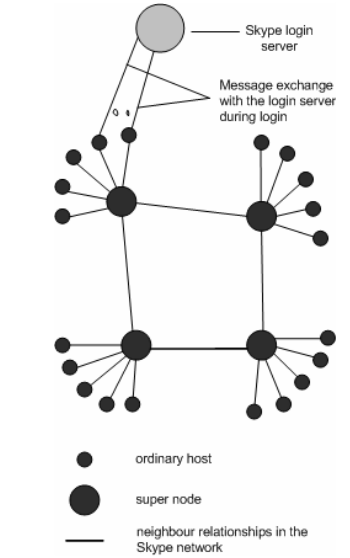
\includegraphics[width=8cm]{fig/skype-architecture.png}
	\caption{Telepathy components registered with user session D-Bus.\cite{skypeProtocolAnalysis}}
	\label{fig:skypeArchitecture}
\end{center}
\end{figure}

\subsection*{Windows Live Messenger}
Windows Live Messenger was first released in July 1999 as MSN Messenger and offered just text messaging with users of AOL Instant Messenger\cite{AIM}. Due to AOL's constant effort to block Microsoft from it's network Microsoft gave in and removed the feature. Since then MSN Messenger could only connect to MSN Messenger Service. In 2001 with the release of Windows XP, MSN Messenger 4.6 came out with voice call support. The last version of MSN Messenger, version 7.5, featured video calls. Windows Live Messenger 8.0 was released in june 2006 and that was the end of the name MSN Messenger.   

Windows Live Messenger utilizes client-server model and communicates using Microsoft Notification protocol over TCP. The first 7 versions of MSNP were disclosed to public, but since version 8 the details have been kept a secret. MSNP does not use encryption so eventhough MSNP's description was not published it was not hard to put it together using packet sniffers.

The live Messenger is available for Windows, Mac OS X and recently was integrated into Microsoft's game console Xbox 360. It features social network integration, offline messaging, games and applications, voice and video calls and standard IM features. An interesting feature is Multiple points of presence allowing user to be connected on two devices. Shared whiteboard is available as an extra application and is not capable of multi-user session.   

\subsection*{Brosix}
An award winning application first released in 2006. Brosix features voice and video chat and multi-user chat, basic IM functions and couple advanced functions. Brosix's whiteboard is an Microsoft Paint like window shared among the participants and won Best IM Feature 2009 award from about.com. Next great feature allows users share screen, including mouse and keyboard much like VNC. Finally Brosix implements co-browsing where users share a browser window. 

Brosix is available for Windows, Max OS X and GNU Linux in commercial and personal(free) version. There is little known about used technologies and it is almost impossbile to reverse-engineer using packet sniffers as Brosix uses 256 bit AES encryption.

\subsection*{Yahoo! Messenger}
Yahoo! Messenger is just like all of the above a closed program though some information has leaked\cite{wikipediaYahoo}. Yahoo! Messenger protocol(YMSG) uses TCP on port 5050 or a different one if default is unavailable. To get to clients behind firewall HTTP is utilized. Video and voice supposedly use SIP and H.323.

Besides the standard set of IM functions Yahoo! Messenger can call PSTN, send SMS and handle voice conference. Whiteboard feature is called Scribbler and is plugin. Linux is missing in the list of supported platforms while Windows and Mac OS X are not.

\subsection*{AOL Instant Messenger}
AIM is yet another IM with proprietory communication protocol. Though AIM is a bit of an exception for it supports two protocols. First is just for simple text messaging called TOC and has been disclosed to public. Second protocol that supports all of the advanced features is being kept a secret.

AOL's messenger is available for Windows and Mac OS X and features voice and video calls as well as whiteboarding. Whiteboard is available as a plugin for AIM called IM Whiteboard. 

\section{Multimedia streaming protocols}
The following section lists the most popular protocols for VoIP work and explains how it works. The first part is about signaling protocol SIP and the second about streaming protocol RTP.

\subsection*{SIP}
Session Initiation Protocol is standardized by IETF and was firts defined in RFC 2543. The latest definition is in RFC 3261. SIP is used in VoIP for negotiating the details of the call. The parameters of the call are described using Session Description protocol described in RFC 4566. Though designed for VoIP it can be used for establishing or terminating any kind of session whether it is between two users or it is a multiuser session. Among the features of SIP is also instant messaging, presence or any kind of event notification. SIP uses primarily UDP on port 5060, but can also use TCP on the same port and 5061 for TLS secured SIP. The syntax is similar to HTTP.

SIP clients are identified by URI which usualy looks like this: \verb|sip:username@hostname|, to be concrete \verb|sip:bob@biloxi.com|. Firts the client must register with a SIP proxy, which in Bob's case is \verb|biloxi.com|. Now let's say Alice wants to call Bob. Todo that she needs to know his URI. She sends an \verb|INVITE| to her SIP proxy, by which it is forwarded to Bob's proxy and finally delivered to Bob and his phone or computer start ringing. If he picks up an appropriate numeric code is sent to Alice. The following example\cite{SIPRFC} shows the scenario presented:    

\begin{figure}[h]
\lstset{language=XML,caption={SIP invite from Alice to Bob}, label=lstSIPInvite}
\begin{lstlisting}
INVITE sip:bob@biloxi.com SIP/2.0
Via: SIP/2.0/UDP pc33.atlanta.com;branch=z9hG4bK776asdhds
Max-Forwards: 70
To: Bob <sip:bob@biloxi.com>
From: Alice <sip:alice@atlanta.com>;tag=1928301774
Call-ID: a84b4c76e66710@pc33.atlanta.com
CSeq: 314159 INVITE
Contact: <sip:alice@pc33.atlanta.com>
Content-Type: application/sdp
Content-Length: 142
\end{lstlisting}
\end{figure}

Since SIP serves only to initiate the session it need to cooperate with a protocol that does transfer the data. That protocol is Real-time Transfer Protocol.  

\subsection*{RTP}
Real-time Transport Protocol is an IETF standard for tranporting data that need to be delivered in real-time rather than reliably. Therefore UDP is used on the transport layer. First was RTP defined in RFC 1889 in 1996 and then later updated in RFC 3550 in 2003. It is primary protocol for streaming audio and video over the internet. It is used for VoIP for transporting the voice while SIP or anoteher signaling protocol negotiates parameters of the transport. More and more TV stations have been converting to the internet and they use RTP as means of distribution. RTP uses unicast as well as multicast when streaming to multiple subscribers.

RTP is used in conjunction with Real-time Transport Control Protocol. RTCP monitors QoS, statictics of the transfer and help with synchronisation when streaming to multiple destinations. The volume of RTPC traffic should be aroung 5\% of the volume of the stream.  

Unlike the circuit switched network, where the QoS is ensured by it's nature, the packet switched network does not have a way of ensuring short or not even constant delay or sufficient bandwidth (it is possible, but very rarely and in private network with proper SLA\footnote{Service Level Agreement}). RTP defines mechanisms for making the most of the packet switched network. It is important to note that in the internet packets of the same stream might take different path to their destination. That and network congestion are the reasons for varying delay commonly reffered to as jitter. RTP labels all the packets with sequence numbers. The implementation of RTP at the destination has a buffer to compensate for jitter and out-of-sequence delivery. If the packet arrives too late it is dropped. Dropping packets to some point might not even be noticable by the user. 

RTP sends and receives data on even port numbers and the associated RTCP uses the next higher odd port number. An example on an RTP packet follows. 

\begin{figure}[ht]
	\begin{center}
	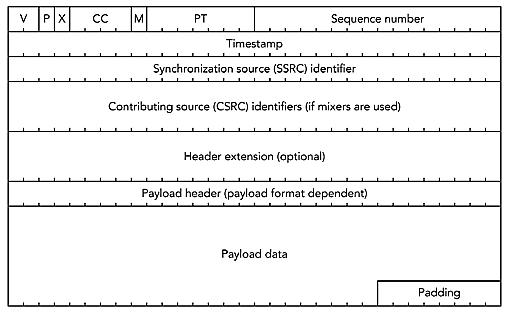
\includegraphics[width=10cm]{fig/rtp-packet.png}
	\caption{RTP packet.\cite{rtpBook}}
	\label{fig:rtpPacket}
\end{center}
\end{figure}


\section{VoIP}
Realization of Voice over IP deals with many problems. Factors effecting voice quality are choice of voice codec, echo cancelation, packetization, packet loss, delay, jitter (delay variation). First the voice needs to be digitized. That is done by a microphone, which consists of anolog-to-digital converter and a mechanism for generating current based on sound in it's proximity. It is important to note that human ear can hear sounds of frequency between 16 to 16000Hz, but only fraction of this spectrum is used when speaking. It is 400 - 3500Hz to be concrete. By recording only a part of the spectrum lower sampling frequency might be used resulting in lower bitrate. The sampling frequency is determined based on Nyquist–Shannon sampling theorem \cite{sampling-theorem}. The AD conversion in digital telephone networks is for example in digital telephone netoworks done by PCM\footnote{Pulse-Code Modulation}, which takes 8000 samples - discrete values on the AD converter. Each sample has 8 bits so the resulting bitrate is 64kbit/s. PCM is for it's high bandwidth consumption and low level of captured information not suitable for VoIP \cite{digitalSpeechBook}. There are alternatives specialised for representing speech, which has certain characteristics whereas PCM is used for any type of sound.  
 
The next step is compressing the recorded voice. There are several compression algorithms. First difference is in length of voice chunks they compress. G.729 takes 10ms as opposed to G.723.1 that takes 30ms. The longer the chunks of voice are the less overhead (IP and Ethernet headers) is sent over the transport media. On the other hand the shorter the length the smaller impact on the conversation should the packet get lost. The compression algorithms used by the voice codecs should ideally lower the data size significantly, while causing short algorithmic delay and taking up insignificant amount of CPU time. Unfortunately there is no codec that would excel in all of the above. Good choice is thus a suitable compromise of the qualities. Since codecs are very hard to compare based on those qualities MOS\footnote{Mean Opinion Score} as means of comparrison attribute. The MOS is a subjective evaluation of quality of voice encoded/decoded by the particular codec on a scale 1-5. The table~\ref{tab:voipCodecs} shows the most popular voice codecs with bitrates and MOS. 

\begin{table}
\begin{center}
\begin{tabular}{|l|c|c|}
	\hline
	\multicolumn{3}{|c|}{\textbf{Voice codecs}}	\\
	\hline
		\textbf{Codec name} & \textbf{Bitrate (kb/s)} & \textbf{MOS} \\
	\hline
	G.711	& 64 & 4.1 \\
	\hline
	G.723.1 & 6.3 & 3.9 \\
	\hline
	G.726 & 32 & 3.85 \\ 
	\hline
	G.729 & 8  & 3.92 \\ 
	\hline
	Speex	& 8/16/32 & unknown \\
	\hline	
\end{tabular}
\end{center}
\label{tab:voipCodecs}
\caption{Voice codecs\cite{voiceCodecs}}
\end{table}
% some codecs may recover from loosing one packet but just one

Once the speech is digitized and encoded it needs to be sent over the network. Since VoIP is an interactive service the latency should be less than 150ms. If the delay is too long the users experience the two conversations effect. The types of delay that need to be taken into account at all times are processing delay, packetization delay serialization delay. The processing delay represents time needed for voice digitization and compression and is codec specific. Packetization delay occurres when the encoded voice is being loaded into packets and depends on how long chunks of speech the particular codec uses. Serialization means sending off the data through the network link and the delay is dependent on the available bandwidth on that link. For links with low bandwidth it is recommended to use codecs with low bitrates. G.729 for example uses voice activity detection and silence suppresion. The caller on the other side then is sent carefully generated comfort noise so that he does not think the call went down. The comfort noise however has much lower bitrate requiring lower bandwidth.

Last and largest portion of the total delay is time of network delivery. We need to account for switching and routing delays, link transmission delays and also for jitter buffer delays. The routing protocols work based on destination address which may, and often does, result in packets of one conversation taking different routes to the caller. Different routes mean different delays - jitter. Jitter buffer is used to accumulate arriving packets and presenting them to the user in the correct order. Since RTP uses sequence numbers it is an easy task to reorder packets. The problem is when packets are delivered too long apart. In that case the missing packet is assumed to be lost for the resulting delay would have a worse effect than the missing packet. Network administrators may influence the network transmission delay using QoS mechanisms such as DiffServ\footnote{Differentiated Services}. DiffServ allows the administrators to give the interactive data like voice and video a higher priority than traffic like emails or HTTP. In order to do so the traffic must be classified and then marked. IPv4 provides means for marking traffic and thus allows using QoS throughout the internet. The edge router through which the traffic enters the autonomous system either trusts the marking of data from a neighboring network or (re)marks the traffic itself. Altough most of the networks utilize QoS there are still some that either don't or have incorrect setup.  

\subsection*{Overcoming NAT and firewalls}
First what is Network Address Translation (NAT) and what is it good for. The internet is based on Internet Protocol version 4. The IPv4 was designed in 1981, when internet was just a pack of machines mostly owned by universities and noone could imagine IPv4 address space\footnote{IPv4 address is a 32 bit number - 4,294,967,296 ($2^{32}$) addresses} could ever be used up. The enormous expansion of the internet cause that the IPv4 addresses were all used up in Februrary of 2011\cite{ianaAddressSpaceReport}. This is where IPv6 comes in offering using 128 bit address and thus offering $3.4\cdot10^{38}$ cardinality of address space allowing anyone to have public IP address. The transition from IPv4 to IPv6 is however costly and complex due to the decentralized nature of the internet.  

To connect new devices to the internet without having to wait for/transition to IPv6 NAT is used. It basically ``hides'' an entire network behind one IP address. This solves the problem problem with insufficient amount of addresses, but creates another problem. The devices behind NAT obtain a private address and can not be connected to directly from the internet. The only device that is directly visible from the internet is one with public IP address. Figure~\ref{fig:nat-diagram} shows the typical home network setup. 

\begin{figure}[ht]
	\begin{center}
	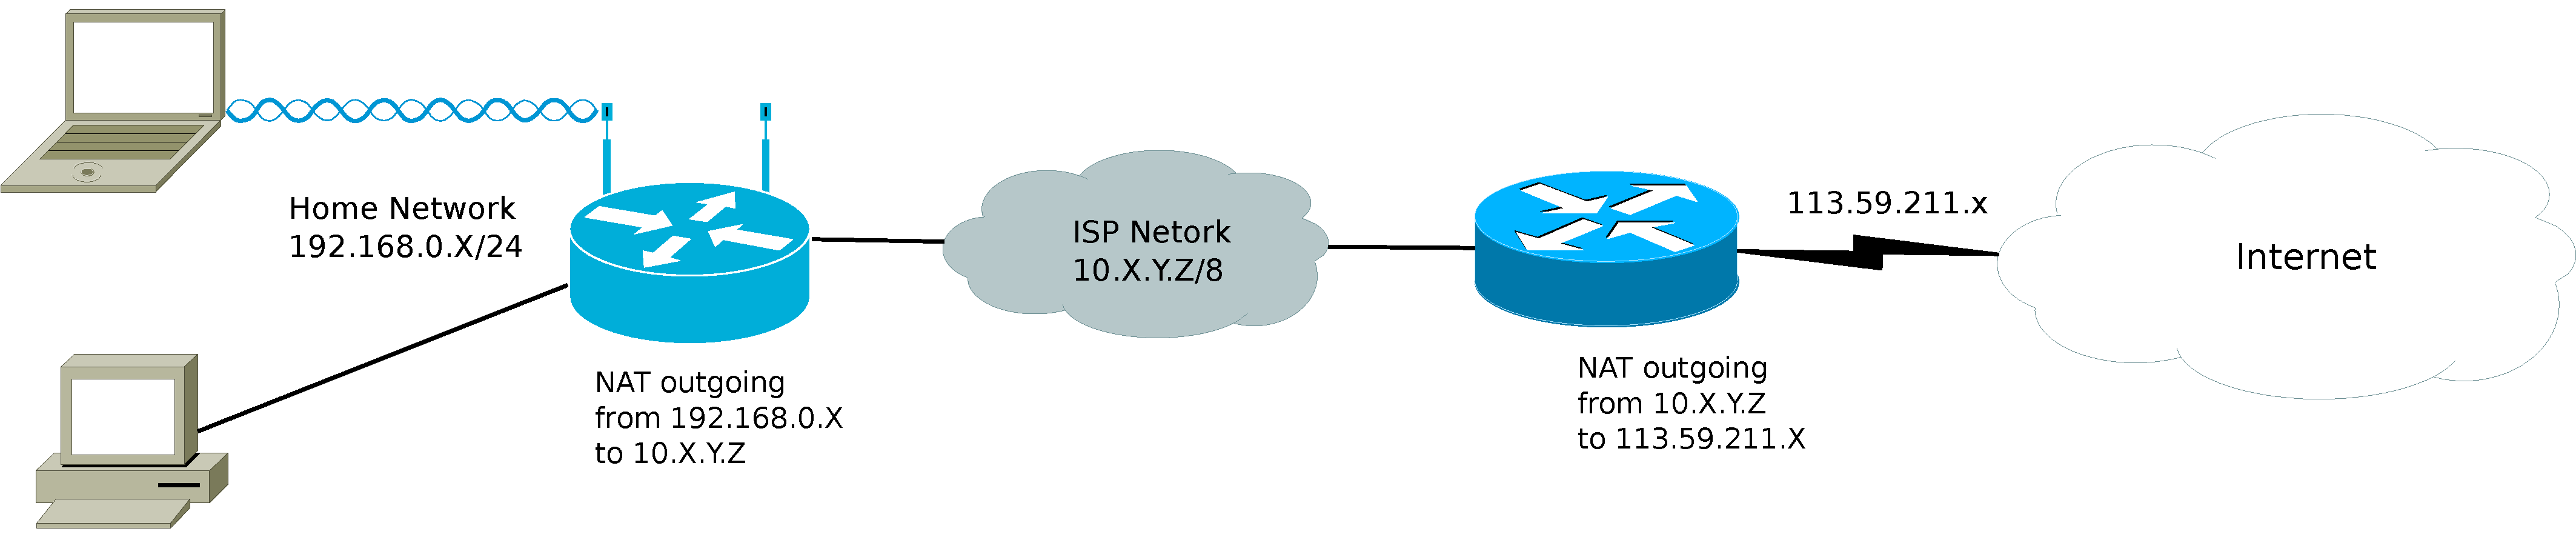
\includegraphics[width=15cm]{fig/nat-diagram.pdf}
	\caption{Typical connection to the internet}
	\label{fig:nat-diagram}
\end{center}
\end{figure}

If a user on the home computer wants look at a website, the home computer sends the request to the router, which performs translation of the home private address to a ISP's network's private address. And the same happens on the edge of provider's network. The routers performing NAT create a mapping of the source IP and source port to translated address and port. The web server sends the reply back to the ISP, with it's address and the translated port number. The edge router looks at mapping and translates back the address and port number and sends it the home router. Same action is performed by the home router and the packets are sent the home computer, which made the request. 

Accessing the home computer from the outside can not be done for two reasons. First private network is not present in the internet's routing tables. And second even if we knew the address of the ISP's edge router, without the dynamic mappings the router would not know which device in it's network to froward the packets to. To summarize it is only possible to send data to a device in a private network if it initiates the communication. Moreso that is possible only if the peer has a public address. Two computers behind NAT can not communicate directly\footnote{It is possible through port forwarding, which is intentionally omitted}.  

There are several solutions for overcoming NAT like STUN or TURN\footnote{Traversal Using Relay NAT} (RFC 5766). STUN is a client-server protocol where the server has a public address and client is behind NAT. Client contacts the server with a request and the server then tries acquire port and IP address, which translate to the client's address and a certain port number. STUN however is not always successful as it can't work with all types of NAT. Next there is TURN, which acts as a relay server and relays traffic from one client to another in case no other mechanism works. It is clear that this is a last resort. Maintaing such servers costs money for the have be connected through links with high bandwidth and the traffic first goes in and then out.

Both of the above mentioned protocols are not universal enough for all kinds address translation systems. Interactive Connectivity Establishment (ICE) by IETF defined in RFC 5245 describes a methodology of taking the best of each NAT overcoming protocol to allow the clients with private addresses to communicate with each other either directly of through third party relay server.  

% =========================================================================================================================
% =========================================================================================================================

\chapter{Port to Telepathy}\label{chapter:port-to-telepathy}
Telepathy communication framework described in detail in chapter~\ref{chapter:telepathy} is a logical choice of communication architecture if one wishes to create a powerful and easily maintainable IM application. A proof that porting to telepathy is a step in the right direction is for example a new client that is being developed by the KDE community and is supposed to become a default KDE IM application. The first release is expected any time now. At that point both main linux window managers KDE and Gnome (Empathy) will have their default IM program based on telepathy. That fact alone promises great and lasting support of this architecture. This chapter talks about the porting of Makneto from iris library to telepathy and explains the design of the application and the reasoning behind it.

The first important change in the architecture of makneto is separation of user interface from the communication backend. There were several reasons supporting this decision. First is that since Telepathy is quite complicated and it takes time to get familiar with it would be best if user interface used a simplified abstraction. And that is where the communication backend comes in. Moreover the backend is the only piece of code that will have to be adjusted should Telepathy undergo any design changes or adjustments. The plan is to make the backend as portable as possible so it could run on most platforms possible. The user interface will be created specificaly for the targeted platform. With that in mind it makes sense to separate backend and frontend. For instead of adjusting user interfaces for all the platforms to the changes the backend will absorb it and frontends will stay unchanged. 

One of the aims of this work is to strip the current application of the iris library and implement the backend based on Telepathy. I chose to use Qt4 bindings for Telepathy simply because the rest of the application was implemented using Qt4 and it is overall very convenient to use with high level of abstraction.	The folowing figure~\ref{fig:MaknetoArchitectureDiagram} shows a diagram of the new Makneto architecture. 

\begin{figure}[ht]
	\begin{center}
	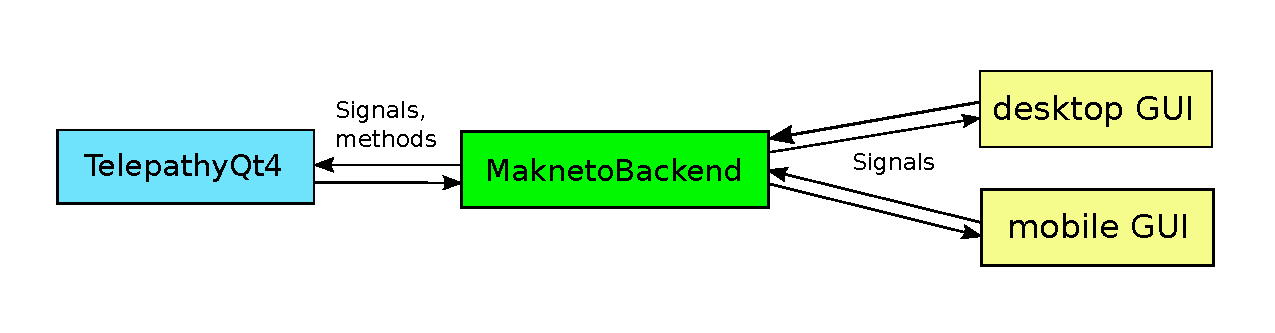
\includegraphics[width=15cm]{fig/maknetoArchitecture}
	\caption{Simplified schema of Makneto components}
	\label{fig:MaknetoArchitectureDiagram}
\end{center}
\end{figure}

\section{Connection}
As mentioned earlier Telepathy communicates over D-Bus, which means that if the application has to have a D-Bus well-known name in order for Telepathy to be able to address it.	Namely the backend needs to implement \verb|Client Handler| interface by subclassing \verb|AbstractClientHandler| and register with D-Bus. Along with wellknown name (in this case Makneto) the application lets telepathy know what channels it is capable of handling. Makneto backend is a Telepathy handler and at this point is able to handle text chat, multiuser chat, audio and file transfer. It is also prepared for video calls, which is functionality outside of the scope of this thesis. More on that in the following chapter. 

Client handler needs to be initialised and that is where the \verb|TelepathyInitializer| class comes in. It merely needs a name of the client and sets up features for contact, connection, account and channel factories. The factories ensure that if the managed object like connection for example is ready it supports all the features specified upon the creation of the connection factory. That way the factories hold the desired features and once the object emits \verb|ready()| signal there is no need to query the available features. The factories are supplied to constructor of Account Manager. Account Manager contains \verb|Account| objects representing accounts of the user. To be able to use Account Manager \verb|becomeReady()| method must be called and then wait for \verb|finished()| singal. Then the accounts may be accessed. The accounts we get from the Account Manager must also be made ready the same way as the manager. Once everything is ready to use the \verb|Initializer| emits \verb|finished()| signal. 

At this point nothing stands in the way of having the accounts go online. This is handled through a context menu of a contact list, see section~\ref{section:contactList} on the frontend and by . When an account is brought online thei Connection Manager creates a Connection with features specified in the ConnectioFactory. If there is another telepathy application already running with the account online the Connection for that account will be shared to prevent wasting resources. 

Figure~\ref{fig:MaknetoBackendClassDiag} shows classes of the Makneto backend that participate on the communication with Telepathy and through it with anyone else. \verb|TelepathyClient| handles both incoming and outgoing  Channels of types asked for upon registration with D-Bus. Once a Channel arrives the \verb|TelepathyClient| checks if a session with the contact already exists and if it does the Channel is handed over to it. If not than new session is created and signal is emitted to inform the user interface. \verb|Session| class encapsulates all of the communication of the user with the outside world. This is the main difference between iris and telepathy. Iris uses a single point of entry for all communication whereas with telepathy it is done via Channels. The session represents all kinds of interaction the user might have with the outside world through Makneto. 

It is important to note that outgoing channels eventhough requested via \verb|Session| invoke \verb|handleChannels()| method of the \verb|TelepathyClient|. There is a flag present with the channel indication whether it has been requested or is coming from the outside. 

\begin{figure}[ht]
	\begin{center}
	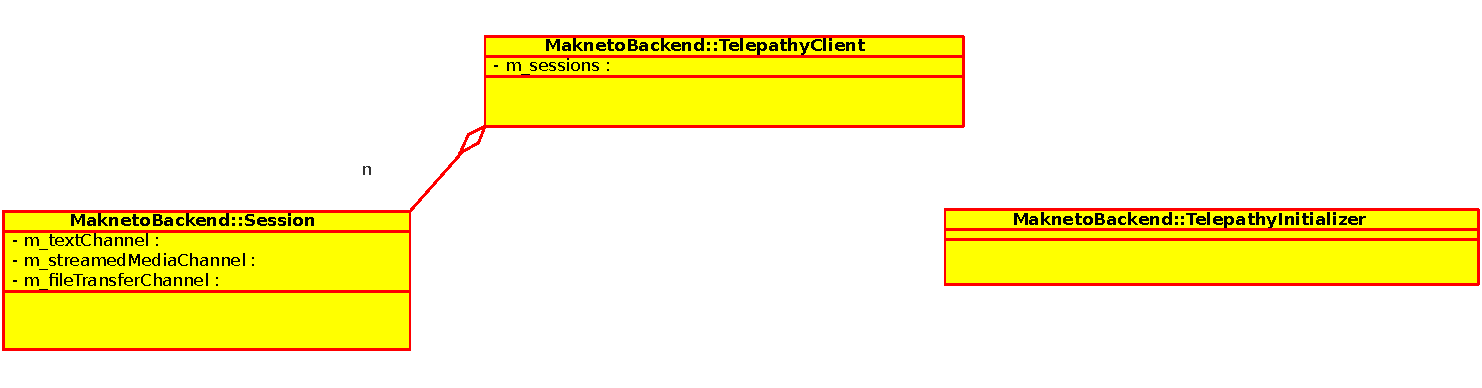
\includegraphics[width=15cm]{fig/makneto-backend-class-diag.pdf}
	\caption{Makneto backend class diagram}
	\label{fig:MaknetoBackendClassDiag}
\end{center}
\end{figure}

\section{Whiteboarding}
Whiteboarding at this point is not supported by Gabble, connection manager for XMPP. Makneto itself the feature supports for it is Makneto's main feature. Until a plugin for whiteboard support is written for Gabble, the whiteboard messages will be tunneled through text messages. The main problem was sending SVG data to clients that would simply display the data to the user. Luckily XMPP offers resource parameter, which is used to check if the contact on the other side is using Makneto and thus can interpret the data correctly. Unfortunately this meant loosing the ability to whiteboard with clients implementing SVGWB by Joonas Govenius, though the JEP has not yet been approved. Whiteboard classes belong to the backend and once the functionality is added to Gabble it will be a simple task to make use of it and restore the lost compatibility. 

The main whiteboarding classes remained unchanged except for the SVG data delivery. The previous implementation based on the iris library supplied conveniently a XML element containing the whiteboard information. Since telepathy does all the XML parsing and interpretation for us, the only option was reconstruct the \verb|wb| element from string.  

\section{Contact list}\label{section:contactList}
Makneto's contact list has been ported to telepathy and utilizes Qt model/view architecture. The model is a part of the backend and the view is a part of the user interface. The contact list model is based on a model from Telepathy-Qt4-Yell project\cite{telepathy-qt4-yell}. The model is connected to all the possible signals stating the item's properties have changed. Once the item has changed, the model's slot receives the signal and emits \verb|changed()| signal, letting the view know it should update information showing to the user.   

One of the greatest benefits of telepathy - multi protocol support - is now present in Makneto. The new contact list model has two types of nodes (items) as shown in the class diagram in figure\ref{fig:contactListClassDiag}. Since it is a tree model I will start from the nodes. Nodes are individual accounts registered with telepathy. These accounts may used in other applications built on telepathy. Leaves are items representing contacts under each account. Although whiteboarding is supported only through XMPP, the other of the features like text chatting or file transfer are available over the other protocols. It must be of course supported by the client of the peer.

As you can see from the class diagram the \verb|TelepathyClient| has an instance of the contact list model. This is useful for requesting sessions with contacts from the frontend - \verb|RosterWidget|. It simply specifies the contact or account by sending index of currently selected item of the model. Any other way would require implementing special Makneto classes for contact and account in order to keep the frontend indenpendent on telepathy   

\begin{figure}[ht]
	\begin{center}
	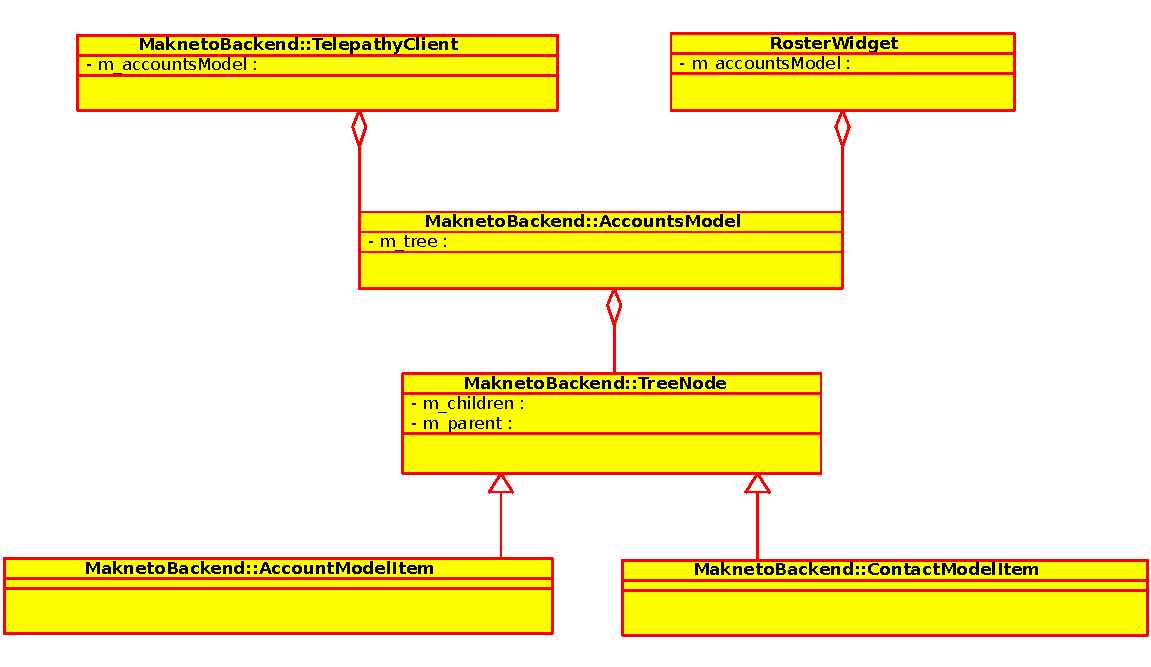
\includegraphics[width=15cm]{fig/contact-list-class-diag.pdf}
	\caption{Makneto contact list class diagram}
	\label{fig:contactListClassDiag}
\end{center}
\end{figure}

The user interface was kept almost the same eventhough both of the communication libraries have very different usage. Moreover this work does not aim at the frontend. One major change of the GUI is worth noting. The main class \verb|Makneto| was an attribute in most of the classes and was passed along trhough all those classes. I have utilized the singleton design pattern, for only one instance of the class exists. Makneto's \verb|Instance()| method is static making it possible to get instance of the class  anywhere within the application. \verb|TelepathyClient| is also implemented as a singleton. 

% =========================================================================================================================
% =========================================================================================================================

\chapter{VoIP implementation}\label{chapter:voip-implementation}
The final chapter of this work contains details about implementation of VoIP into the application Makneto. Frameworks used for handling multimedia are listed with short description. And finally I talk about the implementation itself. Information in this chapter were found at \cite{gstreamer, phonon, farsight} 

Implementing an application handling multimedia means working with devices like sound card, camera, etc. There are several ways of doing so. First would be low-level access, which is platform and device specific. In GNU/Linux it requires using either Open Sound System (OSS) or Advanced Linux Sound Architecture (ALSA). Both of those offer abstraction of hardware beneath, but very low and work only on UNIX like systems and GNU/Linux respectively. Since I am aiming at portability they are not a good choice. Next is using a multimedia framework with higher level of abstraction supported on multiple platforms such as Gstreamer \cite{gstreamer} or Phonon \cite{phonon}.  

\section{GStreamer}
GStreamer is a multimedia framework for writing streaming multimedia applications. It is based on GLib 2.0 and offers API for writing plugins and thus extending it's functionality. Programmers use API for creating applications handling audio, video or both. Recently a stable bindings for Qt have been released making the development even more convenient. Have a look at figure~\ref{fig:gstreamerArchitecture} to get an idea of what the framework consists of.  

\begin{figure}[ht]
	\begin{center}
	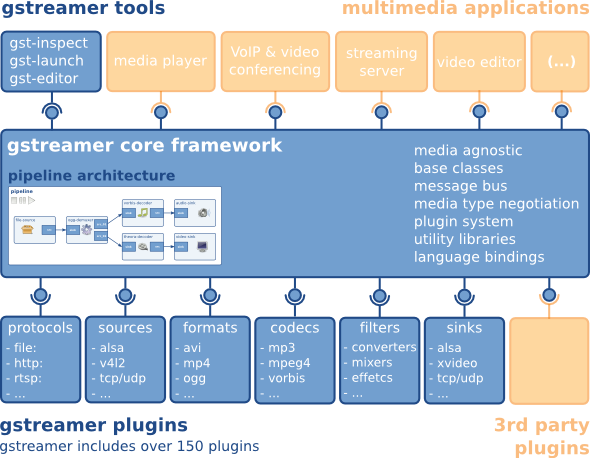
\includegraphics[width=8cm]{fig/gstreamer-architecture.png}
	\caption{GStreamer architecture}
	\label{fig:gstreamerArchitecture}
\end{center}
\end{figure}

Building an application using GStreamer is done by chaining the basic objects - elements. Each element performs a specific function like encoding audio stream, displaying video on the screen on reading from a network stream. It has data inputs and outputs called pads. Depending on the element it might have just an output pad called source\footnote{Source because it is a source from the next element's point of view}. That might be for example one representing an audio file. If it contains just an input pad - sink, then it might be a sound card or screen. Elements containg two pads are filters, encoders, decoders, etc. and more than two would be muxers, demuxers, etc.

Chaining elements to perform certain function means connecting their sources and sinks. The chain is called pipeline and there is an example of one in figure~\ref{fig:gstreamerPipeline}. There are several elements linked together starting with the file-source. The file contains both audio and video and thus a demuxer is used with two sources, one for each stream. Next there is decoding and presenting the result to the user. With a large number of plugins supporting most of known codecs and devices this framework becomes a very powerful tool. 

\begin{figure}[ht]
	\begin{center}
	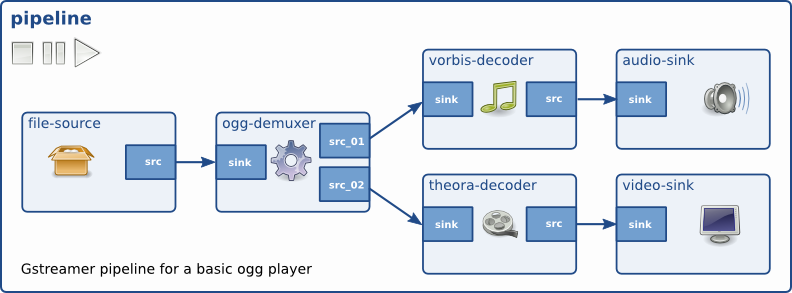
\includegraphics[width=10cm]{fig/gstreamer-pipeline.png}
	\caption{Example of a GStreamer pipeline}
	\label{fig:gstreamerPipeline}
\end{center}
\end{figure}

Pipeline is a special case of bin, which is a collection of elements. Since bin is also an element the programmer can create a pipeline consisting of serveral elements and performing certain function and use it as element in a larger and more complex pipeline. This design allows abstraction on a very high level. When linking elements together the media type that one produces and the other consumes must be compatible. That is determined through elements' capabilities in a process called ``caps negotiation''. GStreamer provides a way of automatic linking of elements called autoplugging based on capabilities. 

When an element is created and linked there is no data flowing until it's state changed to play. The default state in which no recources are allocated is null. Next state is ready, when the element has all of it's resources allocated, but the stream is not opened yet. It is during this phase when the user finds out that the resource is unavailable or incompatible. From ready the elements go to paused by opening the stream a buffering it's contents. At this point the elements should be ready to switch state play instantly. Finally the play state is same as paused, but the data is actually flowing. 

GStream is designed for high performance. Data between elements are copied only when absolutely neccessary, otherwise pointer dereference is used. Moreso the stream processing is running in separate threads.  

\section{Phonon}
\section{Farsight}
%telepathy streamedMediaCall

% =========================================================================================================================
% =========================================================================================================================

\chapter{Conclusion}
The world of today can be described as one enormous network, to which everyone is or soon will be connected. One of the Internet's greatest features is bringing people together. People who hundred of years ago would have to travel sometimes months to see each other or wait for reply get an opinion on an idea from a colleague. Today it is just a few clicks away.

Numerous application exist featuring whiteboard and VoIP and some of them even video conferencing. All of the programs mentioned in chapter 5 unfortunately used proprietory protocols and do not provide any information about it at all. 

There are several ways to implement a VoIP solution. RTP with SIP seems to be a feasible solution as it has been proven to work by numerous applications.Though after much thinking it seems the technologie to with will be XMPP Jingle. It has been implemented by Collabora and is now part of Telepathy Gabble - XMPP connection manager. Though still under development the presented result look promising.

There are several tasks to be done. First is porting Makneto to Telepathy. Then a thourough examination of voice encoding must be done to decide what codec shall be used. And finally implementing VoIP support to Makneto.   



